\documentclass{article} 
% \usepackage[vietnamese]{babel}
\usepackage[utf8]{vietnam}
\usepackage{graphicx}
\usepackage{biblatex}
\bibliography{references.bib}

\graphicspath{{images/}}


\title{Báo Cáo về Phân Lớp Dữ Liệu Bằng Danh Sách Luật Bayesian cho Bài Toán Dự đoán Đột Quỵ}
\author{Nguyễn Hữu Lộc - 23C15031}
\date{31/12/2024}

\pagenumbering{arabic}

\begin{document}

\maketitle

\tableofcontents


\section{Giới thiệu sơ lược}
Với sự phát triển vượt trôi của các mô hình Large Language Model (LLM) trong thời gian gần đây, rất nhiều giải pháp đã được nghiên cứu và thử nghiệm nhằm mục đích tăng hiệu quả cho kết quả đầu ra, và giải quyết những vấn đề khó khăn. Đặc biệt quan tâm hơn cả là việc tính minh bạch của các mô hình LLM đang chịu nhiều chỉ trích do sự hình thành ảo giác trong quá trình suy luận, dẫn tới các phương pháp nhằm bổ sung dữ liệu cho mô hình Retrieval-Augmented Generation (RAG) được ra đời. Tuy nhiên các mô hình RAG lại có mặt hạn chế về cơ chế lấy dữ liệu từ các Cơ Sở Dữ Liệu Vector (CSDLV) một cách chưa thực tế và thường phụ thuộc vào cài đặt cố định, thiếu tính linh hoạt. Trong báo cáo này, nhóm sẽ giới thiệu đến một phương pháp mới có tính linh hoạt cao tên là Sel-Reflective Retrieval-Augmented Generation (Self-RAG) nhằm giải quyết vấn đề trên. Self-RAG sử dụng một mô hình tương tự như các mô hình LLM khác nhưng đã được huấn luyện lại cho phép nó có thể tự nhận xét, đánh giá câu trả lời thông qua các Reflection Token, được đưa vào bộ dữ liệu học nhằm mục đích cho phép mô hình tự đánh giá nếu câu trả lời có cần phải có trích dẫn hay không, và liệu trích dẫn hiện tại có phù hợp hay không. Từ đó, có 2 loại Reflection Token là "Retrieval" và "Critique" sẽ được đưa vào huấn luyện để mô hình tự tạo sinh ra, khác biệt so với các mô hình là truy cứu RAG rồi ghép vào prompt, còn Self-RAG sẽ tự tạo sinh ra lúc cần truy cứu. Đây chính là điểm tạo nên sự linh hoạt cho mô hình và giúp giảm chi phí huấn luyện. Chi tiết quy trình này có thể thấy thông qua phần bên phải của Hình \ref{fig:overview_self_rag}.

\begin{figure} 
    \centering
    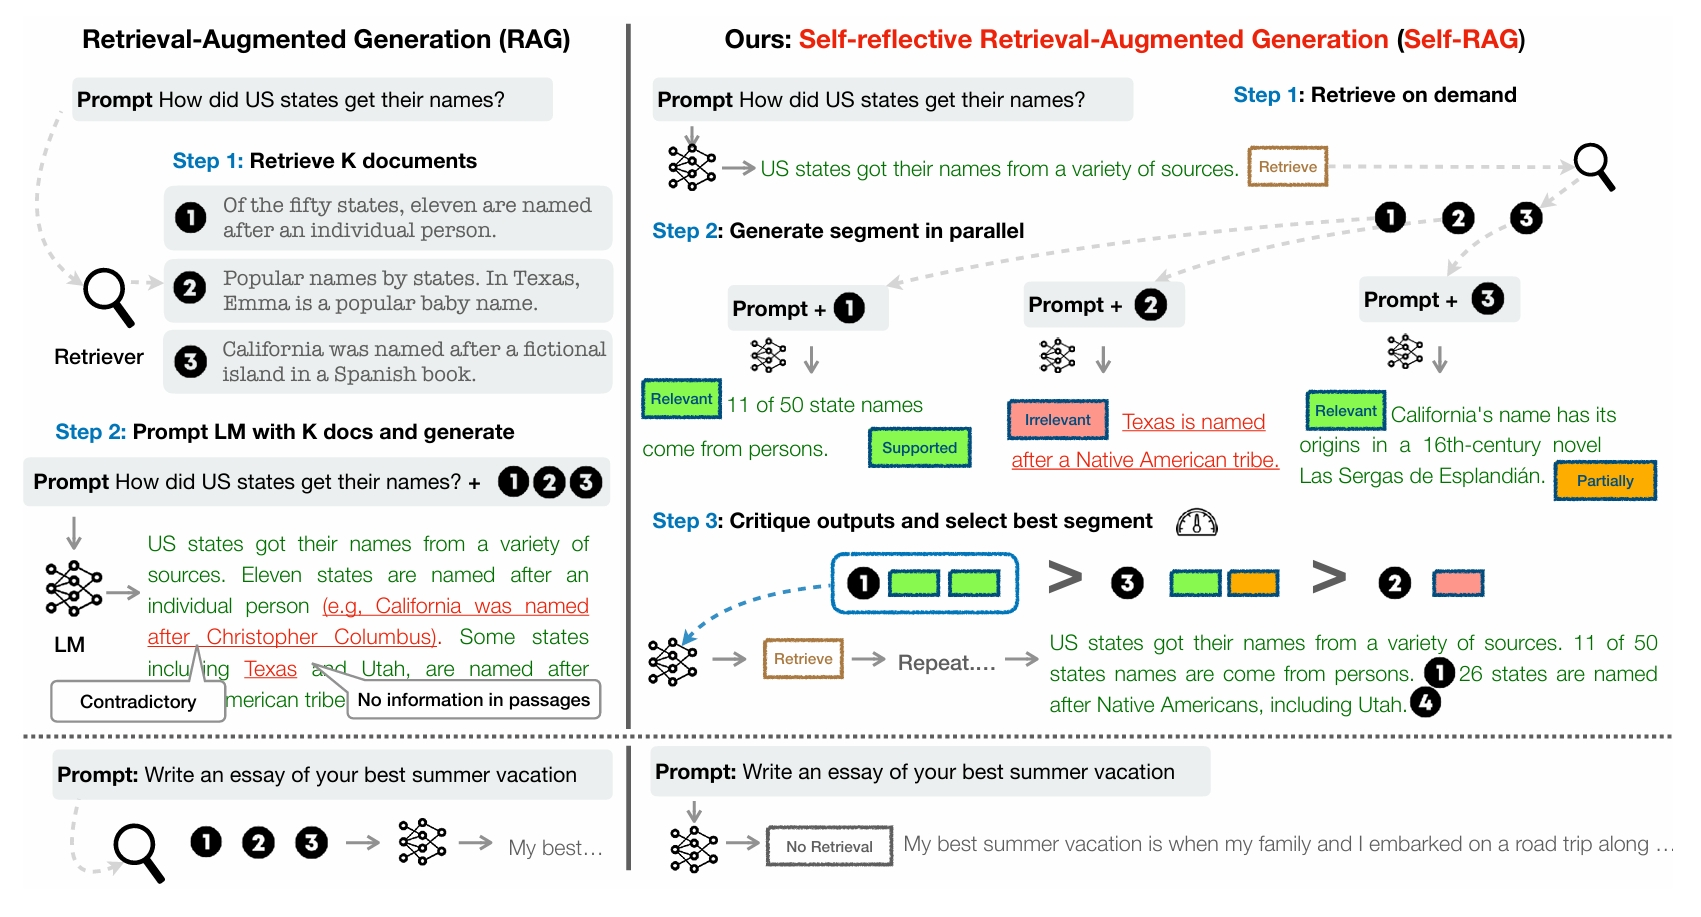
\includegraphics[scale = 0.2]{overview_self_rag.jpeg}
    \caption{Tổng quát sự khác biệt giữa Self-RAG và một mô hình RAG phổ biến.}
    \label{fig:overview_self_rag}
\end{figure}

Để chi tiết hơn thì quy trình của Self-RAG có thể được trình bày như sau: 

\begin{enumerate}
    \item Khi tiếp nhận prompts, mô hình đầu tiên sẽ suy luận nếu nó có cần phải truy cứu dữ liệu từ CSDLV hay không. Nếu cần, mô hình sẽ tạo sinh ra Reflection Token "Retrieval" và gọi truy cứu Retriver. 
    \item Kiểm tra xem các dữ liệu truy xuất ra từ CSDLV có tính liên quan với prompts input hay không và tạo sinh ra các câu trả lời tương ứng với từng dữ liệu. 
    \item Tạo sinh các token "Critique" và kiểm tra kết quả trả lời từ mô hình. Tiêu chí sẽ là tính đúng đắn (factuality) và chất lượng câu trả lời (overall quality) rồi cuối cùng mới trả lại câu prompts output.  
\end{enumerate}

Sự khác biệt của Self-RAG so với các mô hình RAG khác là ở chỗ mô hình sẽ tự tạo sinh ra Reflection Token và token này hình thành thông qua huấn luyện đặc biệt với bộ dữ liệu được xử lý bởi một mô hình "critic" khác. Dữ liệu huấn luyện cho Self-RAG đầu tiên sẽ được đưa qua mô hình "critic" để đánh giá, và thay thế các đoạn dữ liệu thành các Reflection Token "Retrieval" và "Critique" tương ứng, từ đó tạo nên bộ dữ liệu huấn luyện có sẵn những token này. Từ đó, dữ liệu này sẽ được đưa vào huấn luyện, cho phép Self-RAG có thể tự tạo ra những yêu cầu đánh giá và truy vấn theo nhu cầu. Điều này giúp tiết kiệm chi phí thay vì dùng 2 mô hình song song, 1 để tạo sinh câu trả lời và 1 để đánh giá, khi đưa vào thực tế như một vài phương pháp lồng ghép việc đánh giá kết quả từ truy vấn khác như mô hình Adaptive RAG \cite{jeong2024adaptive}. 

Việc sử dụng các Reflection Token cũng cho phép mô hình có sự linh hoạt cao hơn khi có thể cho phép người dùng tạo ra các giới hạn mềm, điều chỉnh số lượng truy vấn hoặc đánh giá theo nhu cầu. Điều này cải thiện được việc thiếu linh hoạt khi điều khiển cứng thông qua điều chỉnh tham số về số lượng truy vấn cho mỗi prompt input như các mô hình RAG ban đầu. 

Trong bài viết này cũng sẽ so sánh kết quả của mô hình với những mô hình phổ biến khác như ChatGPT3.0, Llama2-chat và Alpaca khi chỉ được trang bị cơ chế RAG phổ biến. Bên cạnh đó cũng chứng mình về tính hữu hiệu của việc ứng dụng Reflection token về mặt hiệu quả cả khi huấn luyện và khi suy luận của mô hình.  

\section{Các công trình liên quan}
Các nghiên cứu về RAG gần đây thiên hướng tìm cách để mô hình LLM có thể kết hợp dữ liệu truy xuất một cách nhuần nhuyễn hơn, hoặc tìm cách để tìm dữ liệu từ các CSDLV một cách chính xác, phù hợp hơn để phục vụ prompts input. Gần tương tự như Self-RAG, một vài mô hình cố gắng kết hợp việc truy xuất vào quá trình tạo sinh thay vì chỉ gọi truy xuất cố định vào ban đầu. Tuy nhiên những mô hình đó lại gặp vấn đề về chi phí tính toán và thiếu hiệu quả, dễ gặp vấn đề khi dữ liệu truy vấn thiếu liên quan do cơ chế không đủ linh hoạt, thích nghi kém. 

Một vài nghiên cứu thiên và hướng tinh chỉnh prompt trước khi đưa vào truy xuất nhằm tăng khả năng trả kết quả phù hợp thông qua fine-tune cho mô hình truy xuất và mô hình LLM. Một nghiên cứu dùng các phương pháp suy luận ngôn ngữ, và có mô hình dùng một mô hình tóm tắt (summarization model) để cô đọng thông tin và loại bỏ thông tin dư thừa cũng như tối ưu hóa trước khi đưa vào truy xuất. Dựa trên những ý tưởng trên nhưng hoàn thiện hơn thì Self-RAG cũng fine-tune dữ liệu huấn luyện để tăng khả năng truy xuất nhưng là thực hiện trực tiếp trên mô hình trong lúc suy luận, thay vì cần một mô hình phụ trợ khác. Và Reflection Token cũng giúp tinh gọn những thông tin dư thừa, giúp mô hình tập trung vào những thông tin quan trọng lúc truy xuất dữ liệu. 

Một hướng nghiên cứu khác đang có tính ứng dụng cao là fine tune các mô hình LLM thông qua việc sử dụng phản hồi của người (Reinforcement Learning from Human Feedback) để điều khiển các LLM trả lời, từ đó cho phép mô hình trả lời hiệu quả hơn. Tuy nhiên hướng đi này chủ yếu là giúp tinh chỉnh đầu ra của mô hình theo format mà người thiết kế muốn, hoặc điều chỉnh khả năng suy luận của mô hình hơn là tập trung vào việc trả lời một cách có trọng tâm và có dẫn chứng. Bên cạnh đó, Self-RAG do chỉ chỉnh sửa dữ liệu đầu vào trước khi đưa vào huấn luyện nên chi phí thấp hơn nhiều khi mà RLHF đòi hỏi cần có sự đánh giá của con người với các kết quả tạo sinh.

Nhìn chung thì các nghiên cứu phần lớn đều chú trọng vài bài toán riêng biệt và Self-RAG cũng tương tự như vậy nhưng bổ sung thêm sự cải thiện về độ linh hoạt và chi phí tính toán mà các nghiên cứu khác đang tạm bỏ qua. Trong phần sau nhóm sẽ trình bày cách chi tiết hơn cách mà Self-RAG thực hiện những thay đổi và lý do cho những lựa chọn đó. 

\section{Self-RAG: Học cách tìm nguồn, tạo sinh và đánh giá}

\subsection{Sơ lược bài toán và phương pháp}
Với một mô hình LLM là $\mathcal{M}$ thì khi đưa input là $x$ vào thì mô hình sẽ cần phải tạo sinh ra các output $y$ với $y = [y_1,...y_T]$. Mỗi một $y_t$ có thể là một token trong từ điển hoặc là một token đặc biệt như Reflection Token như đã giới thiệu, và từ đó tự đánh giá hoặc yêu cầu truy vấn để hỗ trợ, làm hoàn thiện câu trả lời hơn. Khi một Retrieve token được tạo ra thì mô hình sẽ cân nhắc việc gọi truy vấn dữ liệu, và đánh giá kết quả của truy vấn có phù hợp để đưa vào chuỗi $y$ hay không. Chi tiết hơn về quy trình này có thể xem tại Hình \ref{fig:self_rag_pseudo_code} và danh sách các Token thì tham khảo ở Hình \ref{fig:reflection_token_explanation}. 

\begin{figure} 
    \centering
    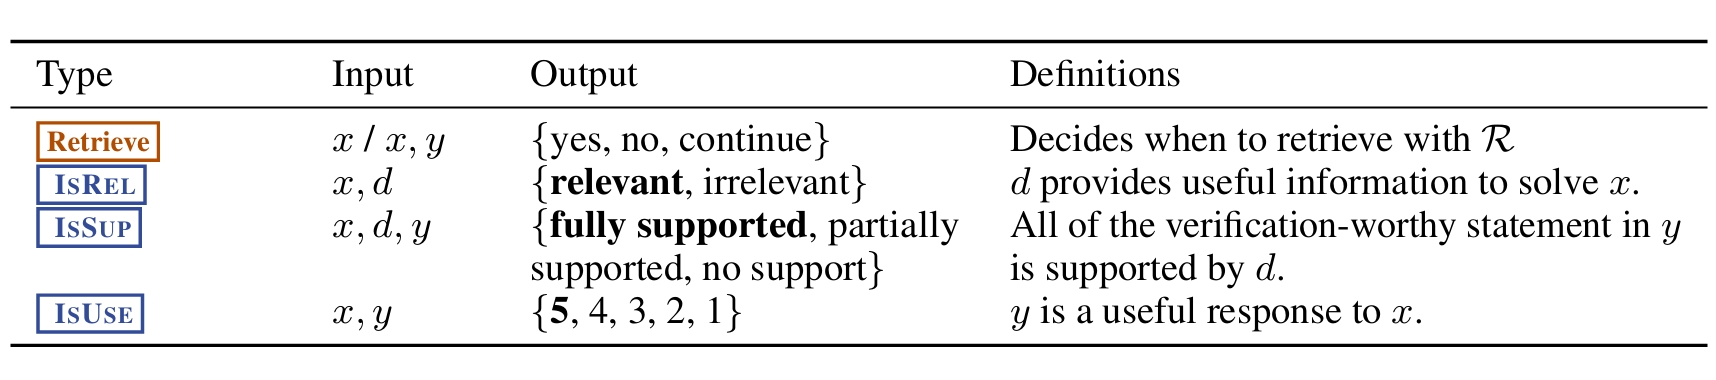
\includegraphics[scale = 0.2]{reflection_token_explanation.jpeg}
    \caption{Các Retrieval Token có thể xuất hiện, đã được cài đặt trong bộ dữ liệu huấn luyện chuyên biệt. Trừ Retrieve thì còn lại là các token bổ trợ cho quá trình đánh giá (Critique). }
    \label{fig:reflection_token_explanation}
\end{figure}

\begin{figure} 
    \centering
    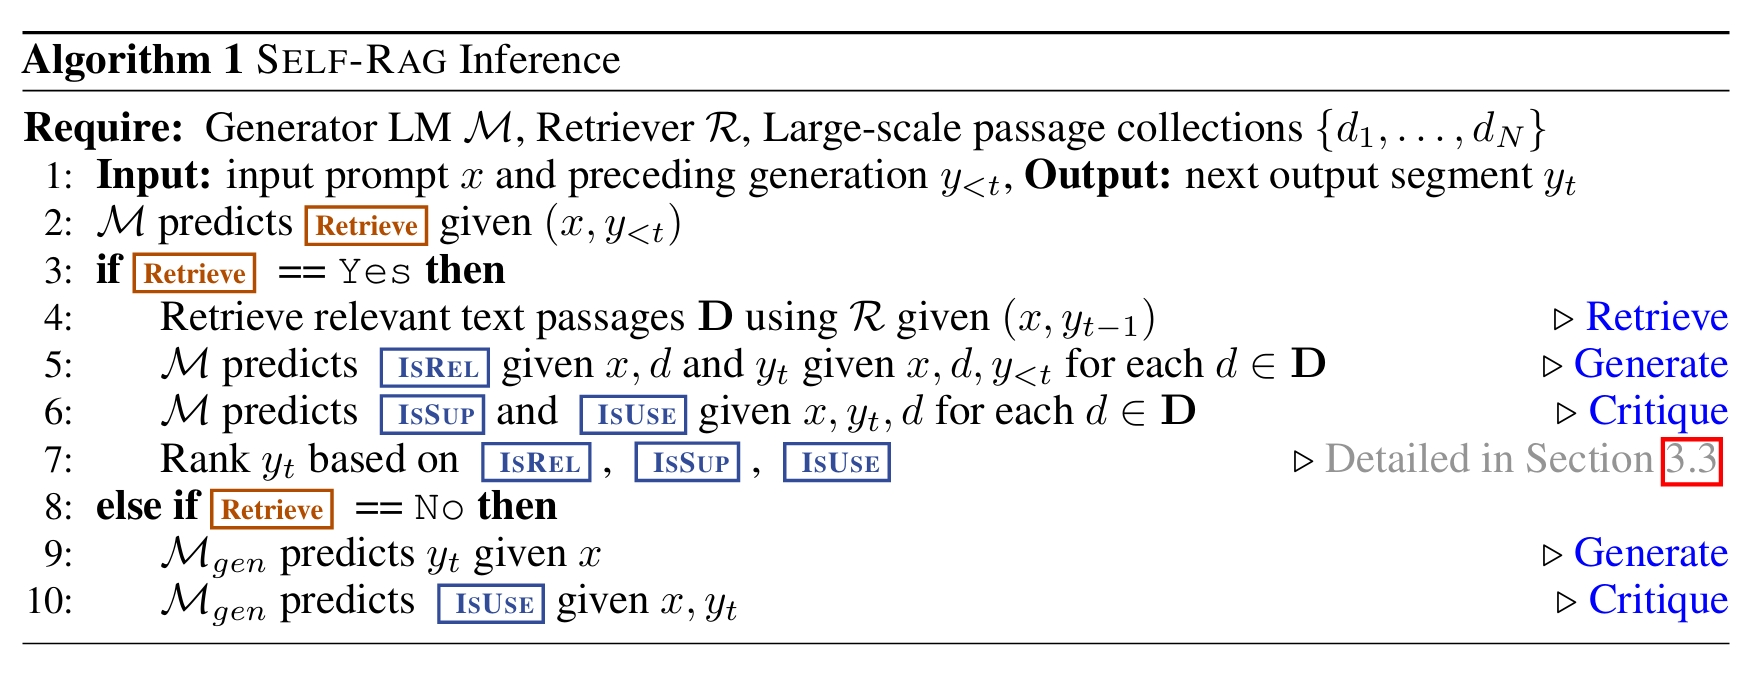
\includegraphics[scale = 0.15]{self_rag_pseudo_code.jpeg}
    \caption{Cách mô hình xử lý khi tạo sinh.}
    \label{fig:self_rag_pseudo_code}
\end{figure}

Thông qua Hình \ref{fig:overview_self_rag} và Hình \ref{fig:self_rag_pseudo_code} thì ta có thể phần nào hiểu được quá trình mô hình Self-RAG hoạt động. Khi mà việc truy xuất để trả lời để không cần thiết, như những lúc câu hỏi thì xoay quanh việc suy luận, thì mô hình hoạt động như mọi mô hình LLM khác, mà ko bị tốn chi phí cho việc truy vấn. Khi truy vấn thì sẽ kèm theo sau đó là phần đánh giá thông qua các token Critique, bao gồm $IsRel$, $IsSup$ và $IsUse$ để kiểm tra tính liên quan, tính hỗ trợ cho trả lời và quyết định có sử dụng hay không. Nếu như nhìn vào ví dụ ở Hình \ref{fig:overview_self_rag} thì văn bản hỗ trợ $d1$ sẽ được lựa chọn do $d2$ không trực tiếp cũng cấp bằng chứng để trả lời và $d3$ chỉ có liên quan một phần. 

Tổng quan về quá trình huấn luyện thì như đã nói sơ ở trên là các Reflection tokens sẽ được tạo ra trong quá trình tạo sinh hoàn toàn tự nhiên, và điều đó dựa trên việc huấn luyện đặc biệt cho mô hình với bộ dữ liệu đã được tinh chỉnh. Chi tiết thì nhóm đã tạo nên bộ dữ liệu (corpus) với các đoạn văn bản được đánh dấu bởi các Retrieve Token để cho mô hình truy vấn $\mathcal{R}$ thực hiện sau. Bên cạnh đó là một mô hình riêng biệt chuyên cho việc đánh giá các đoạn văn bản (critic model) $\mathcal{C}$ sẽ tạo ra các Reflection Token Critique để đánh giá những đoạn văn bản, và nhúng vào trong bộ dữ liệu (corpus) để mô hình học được những điểm sẽ bị đánh giá. Từ 2 phương pháp trên, mô hình $\mathcal{M}$ có thể học được cách tạo sinh ra token để truy vấn và đánh giá ngay trong lúc tạo sinh. 

\subsection{Huấn luyện Self-RAG}
Trong phần này nhóm sẽ miêu tả quá trình huấn luyện 2 mô hình sẽ được sử dụng, đầu tiên là mô hình đánh giá $\mathcal{C}$ dùng cho việc đánh giá các đoạn văn bản và gắn các Reflection Token vào bộ dữ liệu huấn luyện. Kế tiếp sẽ là mô hình tạo sinh $\mathcal{M}$ huấn luyện trên bộ dữ liệu đã được tinh chỉnh.

\subsubsection{Huấn luyện phần đánh giá}
Việc gắn nhãn bằng tay cho các đoạn văn bản là một công việc tốn kém và không hiệu quả, do đó một vài nghiên cứu đã chuyển hướng ứng dụng các mô hình LLM tân tiến như mô hình GPT-4 để phục vụ cho các tác vụ này. Tuy nhiên chi phí cho việc gọi các mô hình như vậy vẫn rất cao và không hiệu quả, dẫn đến một phương pháp mới được đề cập nhiều hơn trong thời gian qua là "model distillation", một phương pháp liên quan đến việc huấn luyện mô hình mạng nơ-ron mới với kích thước nhỏ hơn nhưng vẫn giữ được hiệu suất tương đương với mô hình gốc. Chính xác hơn thì nhóm đã prompt mô hình GPT-4 với hướng dẫn chi tiết ("Given an instruction, make a
judgment on whether finding some external documents from the web helps to generate a better
response.") kế tiếp theo sau là một vài mẫu $I$ gồm input $x$ và output $y$. Với việc dđánh giá bằng tay thì cách đánh giá của GPT-4 rất gần gần với con người, và với 4 đến 20 nghìn mẫu dữ liệu cho mỗi loại như vậy đã kết hợp vào để tạo ra bộ dữ liệu huấn luyện cho mô hình $\mathcal{C}$. Với phương pháp này thì mô hình đánh giá $\mathcal{C}$ có thể sử dụng từ những mô hình khác, không nhất thiết là GPT-4, ví dụ như Llama2-7B, etc. và ước tính có thể đạt được tới 90\% hiệu năng so với mô hình gốc, từ đó làm nền cho phát triển mô hình Self-RAG. 

\subsubsection{Huấn luyện phần tạo sinh}
Đầu tiên sẽ là giao đoạn thu thập dữ liệu cho mô hình tạo sinh, với một cặp input-output $x,y$ thì sẽ được đưa qua mô hình đánh giá $\mathcal{C}$ để đánh giá và tạo ra các Reflection Token xem liệu có cần phải truy vấn dữ liệu hay không. Nếu cần thì mô hình truy vấn $\mathcal{R}$ sẽ được gọi và trả về các kết quả $\mathcal{D}$ và từ đó $\mathcal{C}$ sẽ đánh giá mỗi đoạn truy vấn trả lại và ước lượng nếu như là có liên quan, hỗ trợ hay không với các Critique Token, và cuối cùng sẽ tổng kết mẫu nào sẽ được sử dụng. 

Từ đó, mô hình $\mathcal{M}$ sẽ được huấn luyện trên bộ dữ liệu đã được tinh chỉnh, và từ đó mô hình sẽ học được cách tạo sinh văn bản và thêm nữa là tạo ra các Reflection Token một cách tự nhiên, thay vì chỉ sinh ra những từ ngữ tự nhiên. 

Một vài nghiên các có đưa việc đánh giá vào quá trình huấn luyện có thể nhắc đến là việc sử dụng đánh giá từ con người (Reinforcement Learning from Human Feedback - RLHF) thông qua các Policy để tối ưu hóa độ gần (Proximal Policy Optimization). Tuy nhiên phương pháp này có chi phí cao hơn hẳn so với việc đưa các token đặc biệt vào thẳng quá trình tạo sinh, cho phép mô hình tự đánh giá câu trả lời tốt hơn ngay trong lúc tạo sinh. 

Nhưng nhìn lại thì hướng đi dùng Reinforcement Learning cũng là một hướng vẫn còn đang phát triển, và phổ biến nhất trong hiện tại chính là mô hình DeepSeek chính là dùng các phương pháp điều chỉnh Policy (Group Relative Policy Optimization) vào việc đưa ra mô hình DeekSeek R1 có độ hiệu quả rất cao trong việc suy luận \cite{guo2025deepseek}. 

\subsubsection{Cách Self-RAG Suy Luận}
Việc tạo các Reflection Token trong quá trình tạo sinh trực tiếp cho phép mô hình biến đổi linh hoạt hơn, phục vụ tốt yêu cầu phải đa dạng tác vụ. Với những trường hợp ưu tiên tính chính xác thì mô hình sẽ truy vấn nhiều hơn để đưa ra những câu trả lời sát với thực tế. Còn khi gặp những tác vụ mở, chưa rõ ràng như là soạn ra các đoạn văn bản cá nhân thì mô hình chuyển đổi linh hoạt qua việc giảm truy vấn, ưu tiên tính sáng tạo. 

Để cho mô hình hoạt động linh hoạt được như vậy thì là một vài phương pháp được đưa vào. Đầu tiên là việc cho cho phép người dùng đặt ra các định mức truy vấn (threshold) thay vì để cho mô hình tự yêu cầu truy vấn. Từ đó có thể điều khiển chi tiết cách mô hình tạo sinh. Bên cạnh đó là việc cách Critique Tokens được sử dụng và tính toán, ở mỗi phân đoạn bước $t$ và có yêu cầu truy vấn, thì mô hình truy vấn $\mathcal{R}$ sẽ tìm về $K$ đoạn văn bản và mô hình $\mathcal{M}$ sẽ xử lý chúng song song với $K$ ứng viên kết quả. Khi đó ở mỗi bước $t$ thì ta sẽ thực hiện phương pháp Beam Search để tìm ra kết quả tốt nhất, phương pháp này đánh giá ứng viên thông qua điểm số $\mathcal{S}$ là tổng theo trọng số chuẩn hóa theo xác suất của các Critique Tokens, bao gồm các token (bao gồm $IsRel$, $IsSup$ và $IsUse$). Trọng số của các token đó có thể được điều chỉnh thông qua việc điều chỉnh siêu tham số $w^G$ để cho phép đặt độ ưu tiên cao hơn cho $IsUse$ khi cần các đoạn văn bản truy vấn chính xác hơn. 

\section{Thí nghiệm}

\subsection{Bài toán và dữ liệu}
Để đánh giá một cách khách quán thì nhóm đưa ra một nhóm các bài kiểm tra đa dạng để có thể xác định và khảo sát được các đặc tính của một mô hình tốt như là tính chính xác, sự lưu loát và liệu câu trả lời có dựa trên sự thật. Bên cạnh đó cũng sẽ có những thí nghiệm về Zero-shot learning khi mà các hướng dẫn được đưa ra và không có ví dụ cụ thế. Chi tiết hơn về các bộ dữ liệu và tác vụ thử thách sẽ như sau: 

\begin{itemize}
    \item \textbf{Tác vụ đóng}: bao gồm 2 bộ dữ liệu, một là về kiểm tra độ chính xác dữ liệu y khoa cộng đồng (PubHealth), hai là một bộ trắc nghiệm suy luận kiểm tra khoa học (ARC-Challenge). Độ chính xác sẽ là trọng tâm chính của tác vụ này. 
    \item \textbf{Tạo sinh ngắn}: bao gồm hai bộ dữ liệu trả lời câu hỏi trong miền mở, PopQA và TriviaQA-unfiltered, và mô hình sẽ trả lời các câu hỏi về tri thức thực tế. Đối với PopQA, chúng tôi sử dụng tập con gồm 1.399 truy vấn liên quan đến các thực thể hiếm, những trang Wikipedia có số view thấp dưới 100. Vì tập kiểm tra của TriviaQA-unfiltered không được công khai, nhóm sử dụng tập kiểm tra và tập xác thực từ các nghiên cứu trước đây, bao gồm 11.313 truy vấn. Tiêu chí đánh giá hiệu suất cho phần này sẽ dựa trên việc các câu trả lời chủ chốt (gold answer) có xuất hiện trong kết quả của mô hình hay không, thay vì yêu cầu phải trùng khớp chính xác từng chữ.
    \item \textbf{Tạo sinh dài}: bao gồm tạo sinh tiểu sử và trả lời câu hỏi dạng dài. Nhóm sử dụng FactScore để đánh giá tiểu sử và áp dụng các chỉ số như độ chính xác, độ trôi chảy và độ phủ của trích dẫn để đánh giá câu trả lời dạng dài.
\end{itemize}

\subsection{Cơ sở so sánh}
Với các mô hình so sánh không sử dụng truy xuất, nhóm đánh giá các mô hình ngôn ngữ lớn (LLM) mạnh mẽ đã được huấn luyện trước và công khai (Llama2 7B, 13B), các mô hình điều chỉnh theo hướng dẫn (Alpaca 7B, 13B) và các mô hình được huấn luyện và tăng cường bằng dữ liệu riêng (ChatGPT và Llama2-chat 13B). Đối với các mô hình điều chỉnh bằng hướng dẫn, nhóm sẽ sử dụng prompt hệ thống hoặc các hướng dẫn theo định dạng chính thức trong quá trình huấn luyện nếu có.

Còn với các mô hình so sánh có sử dụng truy xuất, nhóm đánh giá các mô hình có bổ sung cơ chế truy xuất trong quá trình kiểm tra hoặc huấn luyện. Đầu tiên là các mô hình RAG tiêu chuẩn mà các mô hình ngôn ngữ (Llama2, Alpaca) sẽ được yêu tạo sinh ra output dựa trên input kết hợp với các kết quả truy vấn. Nhóm này sẽ bao gồm luôn cả Llama2-FT tức mô hình Llama2 nhưng đã được tinh chỉnh thông qua huấn luyện thêm trên toàn bộ dữ liệu mà nhóm đã sử dụng, nhưng khác biệt là không gồm các Reflection Token. Ngoài ra, nhóm cũng sẽ báo cáo kết quả của các mô hình có bổ sung truy xuất nhưng được huấn luyện với dữ liệu riêng tư, bao gồm Ret-ChatGPT và Ret-Llama2-chat, cả hai đều áp dụng kỹ thuật mở rộng tương tự, cũng như Perplexity. 

Nhóm thứ hai sẽ bao gồm các mô hình khác được huấn luyện với các kết quả truy vấn, chẳng hạn như SAIL, mô hình đã được tinh chỉnh với bộ dữ liệu huấn luyện của Alpaca kèm theo các tài liệu truy vấn được đưa vào sẵn; và Toolformer, mô hình ngôn ngữ với đặc trưng là khả năng gọi API ví dụ như  API của Wikipedia để bổ sung thông tin.

\subsection{Cài đặt thí nghiệm}
Dữ liệu huấn luyện của nhóm sử dụng đã được đa dạng hóa các cặp input-output với bộ mẫu dữ liệu đã được xử lý của Open-Instruct và các bộ dữ liệu chuyên sâu về tri thức với tổng số là 150.000 cặp. Nhóm sử dụng 2 mô hình Llama2 7B và 13B làm mô hình ngôn ngữ nền cho phần mô hình $\mathcal{M}$ và Llama2 7B làm mô hình đánh giá $\mathcal{C}$. Đối với mô hình truy xuất thì nhóm sử dụng Contriever-MS MARCO được cài đặt mặc định và truy xuất tối đa mười tài liệu cho mỗi truy vấn được gọi bởi mô hình chính. 

Theo cấu hình mặc định, trọng số của các tham số $IsRel$, $IsSup$ và $IsUse$ được cài đặt lần lượt là 1.0, 1.0 và 0.5. Để khuyến khích truy xuất thường xuyên, ngưỡng truy xuất sẽ là 0.2 cho hầu hết các tác vụ và 0 cho phần ALCE do yêu cầu cao về việc trích dẫn. Nhóm cũng tăng tốc suy luận bằng vllm. Ở cấp độ đoạn văn, phần Beam Seach đã đề cập ở trên sẽ sử dụng độ rộng beam là 2, tức là sẽ có 2 ứng viên cho kết quả, còn với tạo sinh ở tầng token, nhóm sử dụng phương pháp giải mã tham lam. Theo mặc định thì năm tài liệu hàng đầu từ Contriever-MS MARCO sẽ được cân nhắc, riêng đối với các tác vụ về tiểu sử và câu hỏi mở, mô hình sẽ sử dụng thêm năm tài liệu hàng đầu được truy xuất bởi một công cụ tìm kiếm trên web. Đối với ASQA, năm tài liệu do tác giả cung cấp từ  GTR-XXL sẽ được sử dụng trên tất cả các mô hình được so sánh để đảm bảo tính công bằng.
\section{Kết quả và Phân tích} \label{sec:ketqua}

\subsection{Kết quả}

\subsection{Phân tích}

\section{Kết luận}


\printbibliography

\end{document}